\chapter{Workflow and System Model}

\begin{figure}[h!]
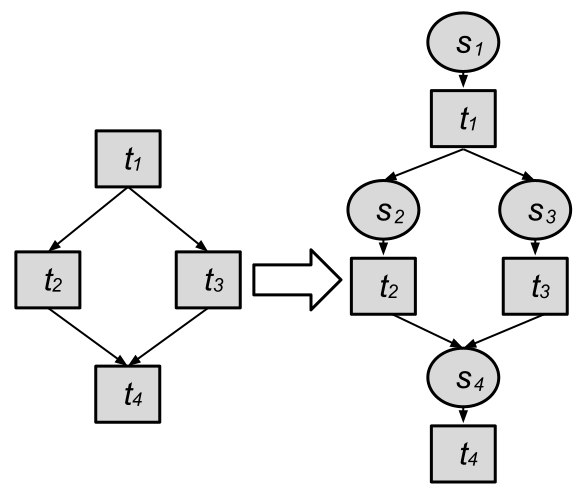
\includegraphics[width=0.5\linewidth]{figures/introduction/odag.png}
\centering
  \captionof{figure}{Extending DAG to o-DAG}
  \label{fig:intro_odag}
\end{figure}

Traditionally a workflow is modeled as a Directed Acyclic Graph (DAG). Each node in the DAG represents a workflow task, and the edges represent dependencies between the tasks ($t$) that constrain the order in which the tasks are executed. Each task is a program and a set of parameters that need to be executed. A job ($j$) is a single execution unit and it contains one or multiple task(s). The dependencies typically represent data flow dependencies in the application, where the output files produced by one task are needed as inputs of another task. In this work, we extend the DAG model to be overhead aware (o-DAG). The reason is that system overheads play an important role in workflow execution and they constitute a major part of the overall runtime when tasks are poorly clustered. Fig~\ref{fig:intro_odag} shows how we augment a DAG to be an o-DAG with the capability to represent scheduling overheads ($s$) such as workflow engine delay, queue delay, and postscript delay. The classification of overheads is based on the model of a typical workflow management system shown in Fig~\ref{fig:intro_system}. The components in this WMS are listed below: 

\begin{figure}[h!]
\centering
  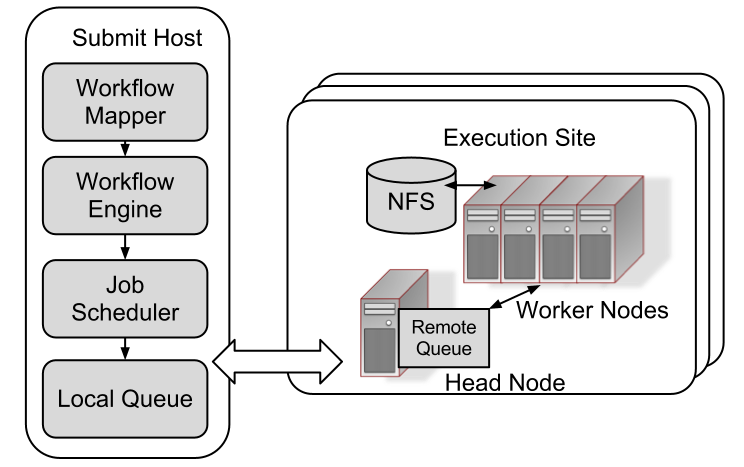
\includegraphics[width=0.6\linewidth]{figures/introduction/system.png}

  \caption{System Model}
  \label{fig:intro_system}
\end{figure}


\textbf{Workflow Mapper} generates an executable workflow based on an abstract workflow provided by the user or workflow composition system. 

\textbf{Workflow Engine} executes the jobs defined by the workflow in order of their dependencies. Only free jobs that have all their parent jobs completed are submitted to  Job Scheduler. 

\textbf{Job Scheduler} and \textbf{Local Queue} manage individual workflow jobs and supervise their execution on local and remote resources.

\textbf{Job Wrapper} extracts tasks from clustered jobs and executes them at the worker nodes. 


\begin{figure}[h!]
\centering
 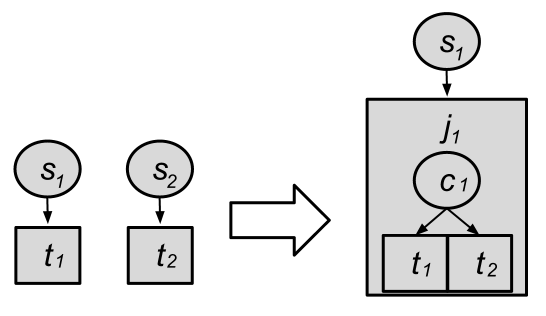
\includegraphics[width=0.6\linewidth]{figures/introduction/hc.png}
  \captionof{figure}{Task Clustering}
  \label{fig:intro_hc}
\end{figure}

%This classification of scheduling overheads is based on our prior studies on workflow analysis \cite{Overhead2011}. 

%Clustering delay ($c$) measures the difference between the sum of the actual task runtime and the job runtime seen by the job scheduler. The cause of clustering delay is usually the use of a job wrapper to execute a clustered job. 
%The job wrapper takes some time to extract the list of tasks and to launch them.

With o-DAG model, we can explicitly express the process of task clustering. For example, in Fig~\ref{fig:intro_hc}, two tasks $t_1$ and $t_2$ without data dependency between them are merged into a clustered job $j_1$. Scheduling overheads ($s_2$) are reduced but clustering delay ($c_1$) is added. 



In this chapter, we first introduce how we extend the existing DAG model to be overhead aware and we also describe the system model that we use in this work. We then analyze the overhead characteristics and distributions across different distributed platforms. Finally we introduce a workflow simulator as an example of the importance of an overhead model when simulating workflow execution. The simulation of a widely used workflow verifies the necessity of taking overhead into consideration. Using our model, the accuracy of runtime estimation can be improved by up to 5 times. 

\section{Motivation}

Traditionally the optimization of workflow performance has been focusing on reducing overall runtime of computational activities through techniques such as  task scheduling that aims to adjust the mapping from tasks to resources. However, these approaches have over-simplified the characteristics of real distributed environments and under-estimated the complexity of large scale workflows. In practice, due to the distributed nature of these resources, the large number of tasks in a workflow, and the complex dependencies among the tasks, significant system overheads can occur during workflow execution. For example, a Montage workflow has around 10,000 tasks, which is a significant load for workflow management tools to schedule or maintain. On one hand, the duration of these tasks is usually around a few seconds, but the system overheads in distributed systems such as Grids can reach up to a few minutes. Merging these short workflow tasks into a larger group of tasks and executing them together can reduce the number of operations (such as job submission) and thus reduce the system overheads significantly. The process of merging tasks into a single job (group of tasks) is called task clustering. 

Task clustering has been widely used in optimizing scientific workflows and can achieve significant improvement in the overall runtime performance \cite{Rynge2012, Singh2008, Li2011, Cao2008} of workflows. However,  there is a lack of a generic and systematic analysis and modeling of task clustering to improve the overall workflow performance including runtime, fault tolerance, data movement and resource utilization etc. To address this challenge, this work extends the existing Directed Acyclic Graph (DAG) model to be overhead aware (o-DAG), in which an overhead is also a node in the DAG and the control dependencies are added as directed edges. We utilize o-DAG to provide a systematic analysis of the performance of task clustering and provide a series of novel optimization methods to further improve the overall workflow performance. 


In this chapter, we introduce our o-DAG model and present our overhead analysis on a series of widely used workflows, which is a base of our optimization methods that will be introduced in the rest of this proposal. 

%\section{Related Work}

%The Directed Acyclic Graph (DAG) has been widely used in many workflow management systems such as DAGMan \cite{DAGMan}, Pegasus \cite{Deelman2004}, Triana \cite{Taylor2006}, DAGuE \cite{Bosilca2011} and GrADS \cite{Cooper2004} . Each node in the DAG represents a workflow task, and the edges represent dependencies between the tasks that constrain the order in which the tasks are executed.  The Directed Acyclic Graph Manager (DAG-Man) \cite{DAGMan} is a service provided by Condor \cite{Frey2002} for executing multiple jobs with dependencies. The DAGMan meta-scheduler processes the DAG dynamically, by sending to the Condor scheduler the jobs as soon as their dependencies are satisfied and they become ready to execute. DAGMan can also help with the resubmission of uncompleted portions of a DAG when one or more nodes resulted in failure, which is called job retry. Pegasus \cite{Deelman2004}, which stands for Planning for Execution in Grids, was developed at the USC Information Sciences Institute as part of the GriPhyN \cite{Deelman2002} and SCEC/IT \cite{Maechling2007} projects. Pegasus receives an abstract workflow description in a XML format from users, produces a concrete or executable workflow, and submits it to DAGMan for execution. 

%A Petri net is a directed bipartite graph, in which the nodes represent transitions and places. The directed arcs describe which places are pre- and/or postconditions for which transitions occurs. Ordinary Petri nets and their extensions have been widely used for the specification, analysis and implementation of workflows \cite{Aalst1998}. Petri nets also enable powerful analysis techniques, which can be used to verify the correctness of workflow procedures. In the scientific workflow community, Petri nets have also been utilized and GWorkflowDL \cite{Vossberg2008}, Grid-Flow \cite{Guan2004} and FlowManager \cite{Aversano2002} are representative examples of this. 

%ASKALON \cite{Fahringer2005} is a Grid environment for composition and execution of scientific workflow applications and uses the standard Web Services Description Language (WSDL) to model workflows. WSDL is an XML format for describing network services as a set of endpoints operating on messages containing either document-oriented or procedure-oriented information. The operations and messages are described abstractly, and then bound to a concrete network protocol and message format to define an endpoint. In ASKALON, the scheduler optimizes the workflow performance using the execution time as the most important goal function. The scheduler interacts with the enactment engine, which is a service that supervises the reliable and fault tolerant execution of the tasks and the transfer of files. 
 
%Compared to these approaches, we extend the original DAG model to be overhead aware so as to analyze the performance of task clustering. An overhead \cite{Prodan2008, Prodan2007} is defined as the time of performing miscellaneous work other than executing the user’s computational activities. In our overhead-aware DAG model (o-DAG), a node can represent either a computational task/job or system overhead during the runtime. A directed edge can represent either a data dependencies between computational tasks/jobs or a control dependency between overheads and computations. Such an extension of the DAG model provides us the ability to model the process of task clustering and analyze the runtime performance of different task clustering strategies. 

%Overheads play an important role in distributed systems. Stratan et al. \cite{Stratan2008} evaluates workflow engines including DAGMan/Condor and Karajan/Globus in a real-world grid environment. Their methodology focuses on five system characteristics: the overhead, the raw performance, the stability, the scalability and the reliability. They have pointed out that head node consumption should not be negligible and the main bottleneck in a busy system is often the head node. Prodan et al. \cite{Prodan2008} offers a complete grid workflow overhead classification and a systematic measurement of overheads. Östberg et al. \cite{Östberg2011} used the Grid Job Management Framework (GJMF) as a testbed for characterization of Grid Service-Oriented Architecture overhead, and evaluate the efficiency of a set of design patterns for overhead mediation mechanisms featured in the framework. In comparison with their work, (1) we focus on measuring the overlap of major overheads imposed by workflow management systems and execution environments; (2) we present a study of the distribution of overheads instead of just overall numbers; (3) we compare workflows running in different platforms (dedicated clusters, clouds, grids) and different environments (resource availability, file systems), explaining how they influence the resulting overheads; and (4) we analyze how existing optimization techniques improve the workflow runtime by reducing or overlapping overheads.


%Fragmentation \cite{Rodríguez2012} is a well known effect in resource allocation, which decreases the resource utilization, as studied in \cite{Smith2000}. Whenever a resource allocation fails, even though enough free capacity is available, fragmentation is easily spotted as cause. In \cite{Gehr2009}, a new way for measuring the fragmentation of a system, as well as their correlation with jobs rejection, is presented. It shows that the proposed fragmentation measure is a good indicator of the state of the system. In this work, we are also interested in the resource under-utilization problem and we use a few cumulative metrics to measure the fragmentation. 


%Performance Analysis of scientific workflows has also been studied in \cite{Rubing2009, Calasanz2008, Truong2004, Uysal1998}. The performance method proposed by Duan et al. \cite{Rubing2009} is based on a hybrid Bayesian-neural network for predicting the execution time of workflow tasks. Bayesian network is a graphical modeling approach that we use to model the effects of different factors affecting the execution time (referred as factors or variables), and the interdependence of the factors among each other. The important attributes are dynamically selected by the Bayesian network and fed into a radial basis function neural network to make further predictions. In comparison, our work in overhead analysis focuses on the relationship between system overheads and the performance of different optimization methods. We investigated a wide range of scientific workflows and analyzed how system overheads influence the performance of optimization of these workflows. 


%Because in Grid systems communication delays are significant all algorithms must achieve maximum parallelism while minimizing data communication. 

%Task Clustering reduces the communication cost and scheduling overheads by grouping the heavily communicating tasks or short runtime tasks to the same job and then assigning the job in a cluster to the same resources. 
%Task clustering algorithms can have two phases: the initial task clustering and a post-clustering phase which can refine the clusters produced in the previous phase. Our work has covered both phases. 

%The low performance of lightweight (a.k.a. fine-grained) tasks is a common problem on widely distributed platforms where the communication overheads and scheduling overheads are high, such as grid systems. To address this issue, fine-grained tasks are commonly merged into coarse-grained tasks \cite{Muthuvelu2005, Muthuvelu2013, Keat2006}, which reduces the cost of data transfers when grouped tasks share input data \cite{Muthuvelu2005} and saves scheduling overheads such as queueing time when resources are limited. However, task grouping also limits parallelism and therefore should be used carefully. Muthuvelu et al. \cite{Muthuvelu2013} proposed an algorithm to group bag of tasks based on their granularity size defined as the processing time of the task on the resource. Resources are ordered by their decreasing values of capacity (in MIPS) and tasks are grouped up to the resource capacity. Then, Keat et al. \cite{Keat2006} and Ang et al. \cite{Ang2009} extended the work of Muthuvelu et al. by introducing bandwidth to enhance the performance of task clustering. Resources are sorted in descending order of bandwidth, then assigned to grouped tasks downward ordered by processing requirement length. Afterwards, Soni et al. \cite{Soni2010} proposed an algorithm to group lightweight tasks into coarse-grained tasks (GBJS) based on processing capability, bandwidth, and memory-size of the available resources. Tasks are sorted into ascending order of required computational power, then, selected in first come first serve order to be grouped according to the capability of the resources. Zomaya and Chan \cite{Zomaya2004} studied limitations and ideal control parameters of task clustering by using genetic algorithm. Their algorithm performs task selection based on the earliest task start time and task communication costs; it converges to an optimal solution of the number of clustered jobs and tasks per clustered job. In contrast, our work has discussed the influence of data dependencies across different levels while they only focus on computational activities (bag-of-tasks). 


%Singh \cite{Singh2008} proposed to use horizontal clustering and label based clustering in scientific workflows to reduce the scheduling overheads in a best-effort approach. The horizontal clustering merges tasks at the same level, while level of a task refers to the distance from a root task to this task using Breadth-First-Search. Label based clustering uses labels set by the users manually and merges tasks with the same labels together. Task clustering strategies have demonstrated their effect in some scientific workflows \cite{Rynge2012, Maheshwari2012, Hussin2010, Liu2009}.  Li \cite{Li2011}  developed algorithm that uses horizontal clustering to group tasks that can be scheduled to run simultaneously. Tasks with the same scheduling priority (determined by the scheduling level) are merged and scheduled to run simultaneously. Cao et al. \cite{Cao2008} proposed a static scheduling heuristic, called DAGMap that consists of three phases, namely prioritizing, grouping, and independent task scheduling. Task grouping is based on dependency relationships and task upward priority (the longest distance form this task to the exit task). Compared to their work, we propose a generic workflow model that takes system overheads into consideration and provide a series of overhead aware task clustering strategies to optimize the overall runtime performance of workflows. 

%Task clustering is one typical category of task scheduling, which maps resources to tasks based on different criteria. List Heuristics assign a priority to a task and the scheduling algorithms attempt to execute the higher priority nodes first. Most scheduling algorithms for Grid systems are based on this approach. For example, scheduling algorithms, such as HEFT \cite{Topcuoglu2002}, MaxMin \cite{Braun2001}, MinMin \cite{Blythe2005}, etc., have been widely used in optimizing the runtime performance of many scientific workflows. Genetic Algorithms \cite{Adamuthe2011} and Neural Network \cite{Babu2012} are also proposed to address the scheduling problem. Compared to them, we aim to generate a group of tasks that are suitable for scheduling and execution while the resource selection is not our major challenge since we already have many mature scheduling algorithms. 




%Pandey et al. (2009) used task clustering to schedule data-intensive tasks for a medical application workflow. They clustered tasks based on their execution time, data transfer and level. If tasks were having high deviation and value of average execution time, they were executed without clustering. Tasks with lower deviation and value of execution time were clustered together. They showed that clustering tasks for data-intensive application workflows has better makespan than scheduling the workflow without clustering, mainly attributed to the decrease in file transfers between tasks in the same cluster.

\section{Approach}

\begin{figure}[h!]
	\centering
    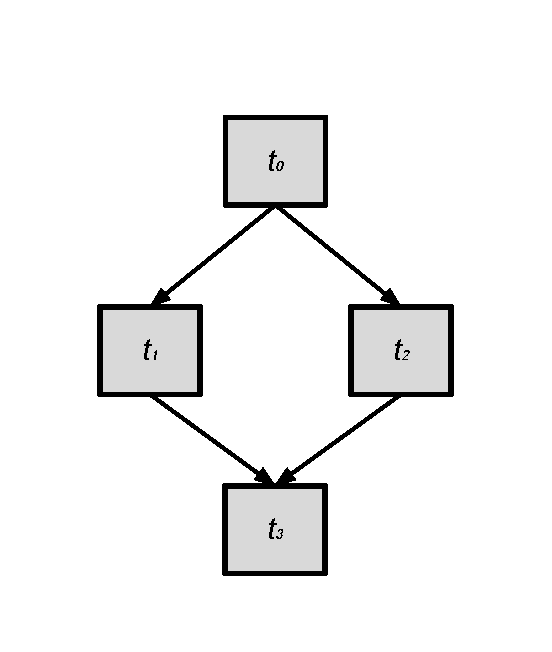
\includegraphics[width=0.5\textwidth]{figures/model/dag.pdf}
    \caption{A simple DAG with four tasks ($t_0$, $t_1$, $t_2$, $t_3$). The edges represent the data dependencies between tasks.}
    \label{fig:model_dag}
\end{figure}

\begin{figure}[h!]
	\centering
    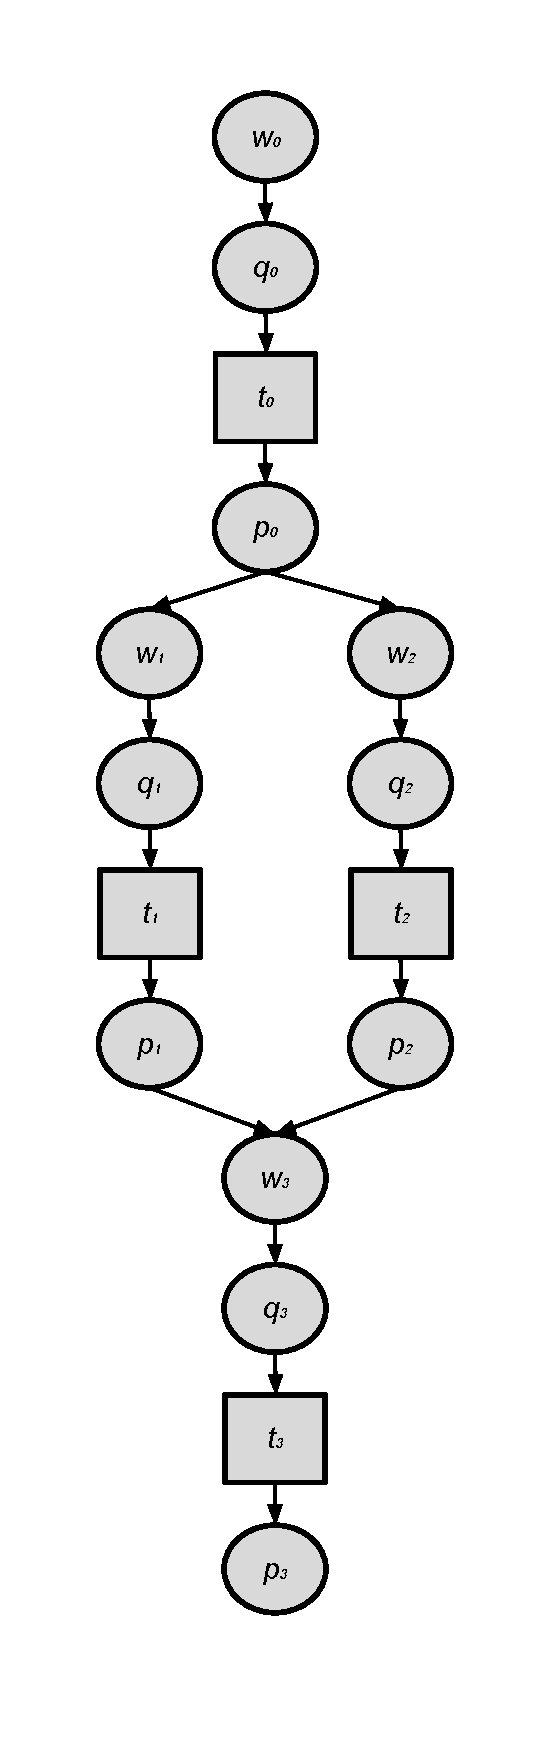
\includegraphics[width=0.4\textwidth]{figures/model/odag_before.pdf}
    \caption{An o-DAG with overheads ($w_0$$\sim$  $w_3$, $q_0$$\sim$  $q_3$, $p_0$$\sim$  $p_3$). The edges represent control dependencies or data dependencies}
    \label{fig:model_odag_before}
\end{figure}

Traditionally a workflow is modeled as a Directed Acyclic Graph (DAG). Each node in the DAG represents a workflow task, and the edges represent dependencies between the tasks ($t$) that constrain the order in which the tasks are executed. Each task is a program and a set of parameters that need to be executed. Fig~\ref{fig:model_dag} shows a simple workflow with four tasks. A job ($j$) is a single execution unit and it contains one or multiple task(s). The dependencies typically represent data flow dependencies in the application, where the output files produced by one task are needed as inputs of another task. 
%In this paper, we extend the DAG model to be overhead aware (o-DAG). The reason is that system overheads play an important role in workflow execution and they constitute a major part of the overall runtime when tasks are poorly clustered. 
Fig~\ref{fig:model_odag_before} shows how we augment a DAG in Fig~\ref{fig:model_dag} to be an o-DAG with the capability to represent scheduling overheads ($s$) such as workflow engine delay ($w$), queue delay ($q$), and postscript delay ($q$). Fig~\ref{fig:model_odag_after} further shows how we perform task clustering in this simple workflow, in which we merge $t_1$ and $t_2$ into a new job $j_4$. The scheduling overheads associated with $t_1$ and $t_2$ are removed and the overheads including the clustering delay ($c_4$) of $j_4$ are added. 

%To execute this workflow, a workflow engine such as DAGMan \cite{DAGMan} processes this DAG starting from the root task ($t_0$) and then executes each task without violating the data dependencies. Take the example of one available resource, a possible schedule would be $t_0\rightarrow t_1\rightarrow t_2\rightarrow t_3$ or $t_0\rightarrow t_2\rightarrow t_1\rightarrow t_3$. Both of the two schedules satisfy the data dependencies are thereby they are correct. 






The classification of overheads is based on the model of a typical workflow management system (WMS) shown in Fig~\ref{fig:model_system}. The components in this WMS are listed below: 




\begin{figure}[h!]
\centering
  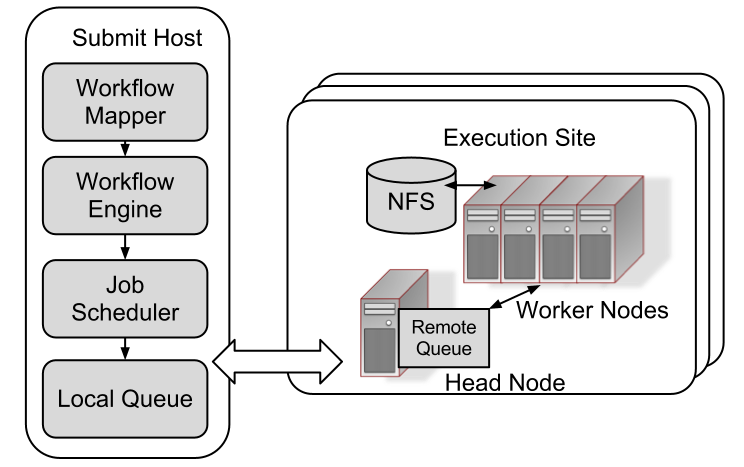
\includegraphics[width=0.6\linewidth]{figures/introduction/system.png}

  \caption{System Model}
  \label{fig:model_system}
\end{figure}


\textbf{Workflow Mapper} generates an executable workflow based on an abstract workflow provided by the user or a workflow composition system. 

\textbf{Workflow Engine} executes the jobs in order of their dependencies. Only free jobs that have all their parent jobs completed are submitted to  Job Scheduler. 

\textbf{Job Scheduler} and \textbf{Local Queue} manage individual workflow jobs and supervise their execution on local and remote resources.

\textbf{Job Wrapper} extracts tasks from clustered jobs and executes them at the worker nodes. 


\begin{figure}[h!]
	\centering
    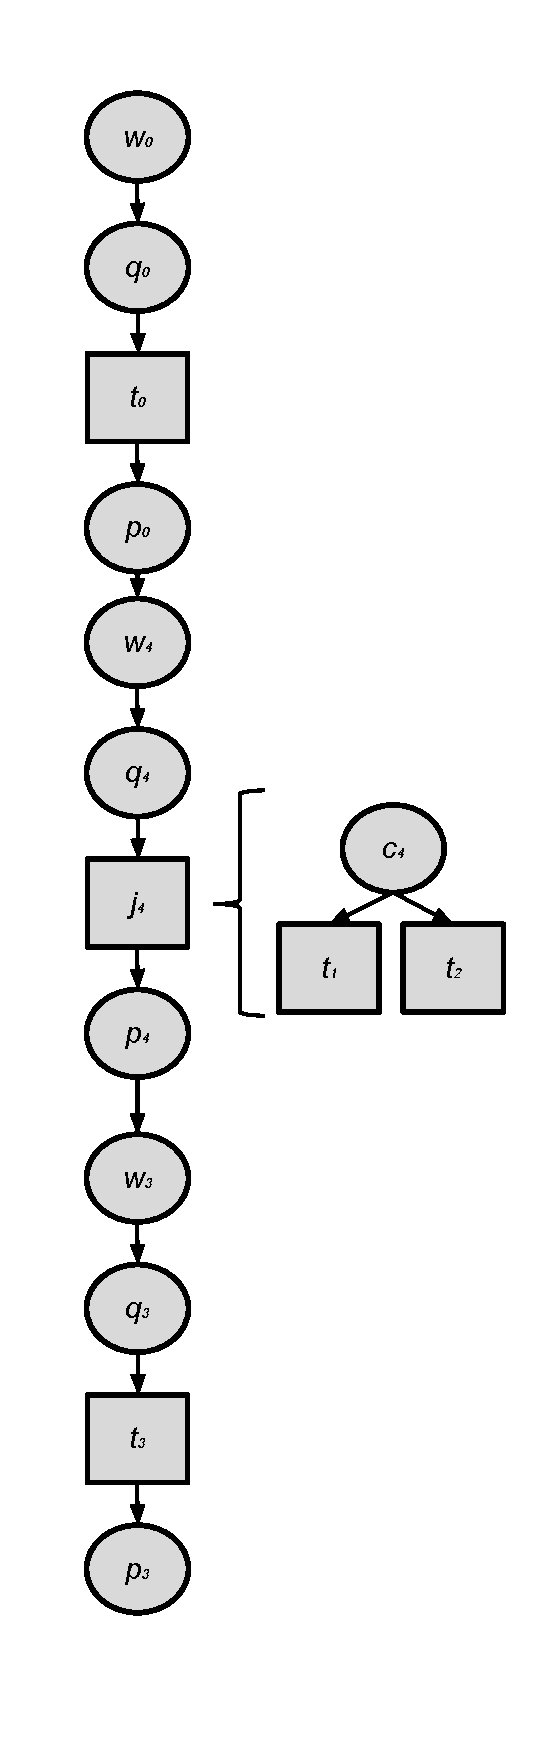
\includegraphics[width=0.4\textwidth]{figures/model/odag_after.pdf}
    \caption{ A Diamond Workflow after Task Clustering}
    \label{fig:model_odag_after}
\end{figure}


%An overhead is defined as the time of performing miscellaneous work other than executing the user’s computational activities. 
%The execution of scientific workflows often suffers from a variety of overheads in the distributed environment. 
%Due to the distributed nature of these resources, the large number of tasks in a workflow, and the complex dependencies among the tasks, significant overheads can occur during the workflow execution. 
%It is essential to identify the different overheads and to evaluate how different optimization methods reduce overheads and improve runtime performance. 
%In this section, we present an overhead analysis for a set of workflows run on cloud, grid, or cluster platforms. 
%We present the overhead distributions and the patterns that they have performed. 

\subsection{Overhead Classification}


\begin{figure}[h!]
	\centering
    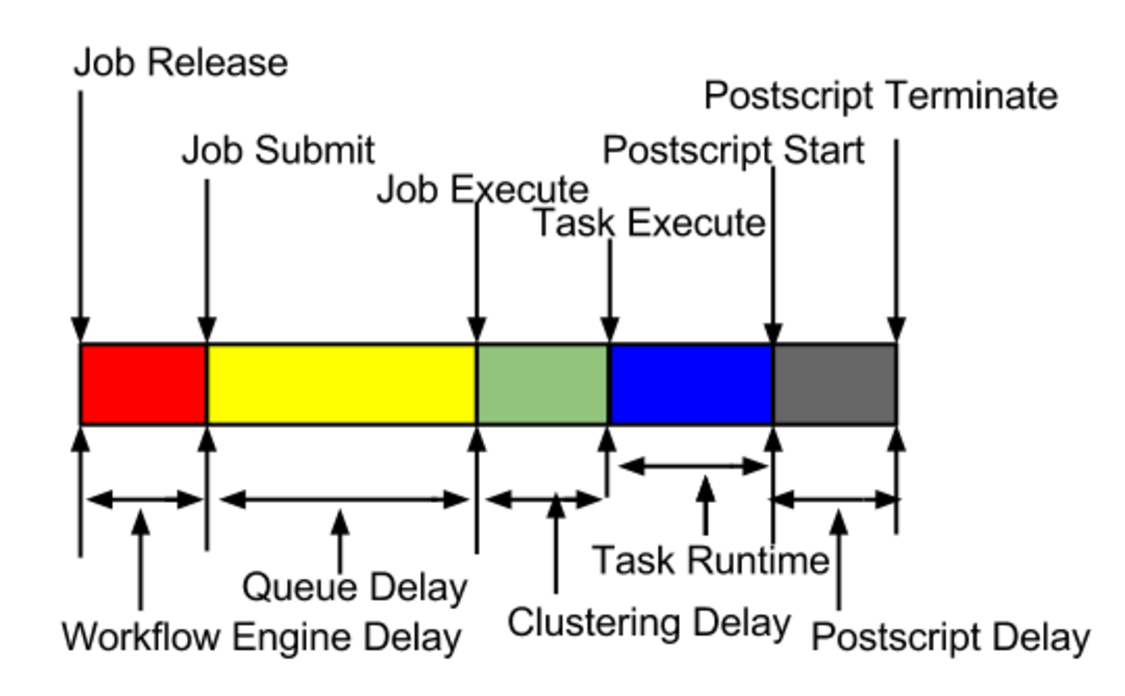
\includegraphics[width=0.7\textwidth]{figures/model/overhead.pdf}
    \caption{Workflow Events}
    \label{fig:model_overhead}
\end{figure}


The execution of a job is comprised of a series of events as shown in Figure~\ref{fig:model_overhead} and they are defined as:
\begin{enumerate}
\item Job Release is defined as the time when the workflow engine identifies that a job is ready to be submitted (when its parents have successfully completed). 
\item Job Submit is defined as the time when the workflow engine submits a job to the local queue. 
\item Job Execute is defined as the time when the workflow engine sees a job is being executed. 
\item Task Execute is defined as the time when the job wrapper sees a task is being executed. 

\item Postscript Start is defined as the time when the workflow engine starts to execute a postscript. 
\item Postscript Terminate is defined as the time when the postscript returns a status code (success or failure). 
\end{enumerate}

Figure~\ref{fig:model_overhead} shows a typical timeline of overheads and runtime in a compute job. We do not specify the data transfer delay in this timeline because data transfer is handled by data transfer jobs (stage-in and stage-out jobs). 

We have classified workflow overheads into five categories as follows. 
\begin{enumerate}

\item{Workflow Engine Delay} measures the time between when the last parent job of a job completes and the time when the job gets submitted to the local queue. 
%In case of retries the value of the last retry is used for the calculation. 
The completion time of the last parent job means this job is released to the ready queue and is waiting for resources to be assigned to it. The workflow engine delay reflects the efficiency of a workflow engine (i.e., DAGMan \cite{DAGMan}). 

\item{Queue Delay} is defined as the time between the submission of a job by the workflow engine to the local queue and the time the local scheduler sees the job running. This overhead reflects the efficiency of the local workflow scheduler (e.g. Condor \cite{Frey2002}) to execute a job and the availability of resources for the execution of this job. 
%The queue delay is an estimate of the time spent in the local queue on the submit host. 

\item{Postscript Delay } is the time taken to execute a lightweight script under some execution systems after the execution of a job. Postscripts examine the status code of a job after the computational part of this job is done.

%\item{Data Transfer Delay} happens when data is transferred between nodes. It includes three different types of processes: staging data in, cleaning up, and staging data out. Stage-in jobs transfer input files from source sites to execution sites before the computation starts. Cleanup jobs delete intermediate data that is no longer needed by the remainder of the workflow. Stage-out jobs transfer workflow output data to archiving sites for storage and analysis.

\item{Clustering Delay} measures the difference between the sum of the actual task runtime and the job runtime seen by the job wrapper. The cause of Clustering Delay is usually because we use a job wrapper in worker nodes to execute a clustered job that requires some delay to extract the list of tasks. 
\end{enumerate}

\subsection{Overhead Distribution}

%We examined the overhead distributions of a wide range of workflows in our experiments . These workflows were run on distributed platforms including clouds, grids and dedicated clusters. 
%%On clouds, virtual machines were provisioned and then the required services (such as file transfer services) were deployed. 
%We examined two clouds: Amazon EC2 \cite{AmazonEC2}  and FutureGrid \cite{FutureGrid}. Amazon EC2 is a commercial, public cloud that is been widely used in distributed computing. 
We examined the overhead distributions of a widely used astronomy workflow called Montage \cite{Berriman2004} that is used to construct large image mosaics of the sky. Montage was run on FutureGrid \cite{FutureGrid}. FutureGrid is a distributed, high-performance testbed that provides scientists with a set of computing resources to develop parallel, grid, and cloud applications. 
%%On grids, grid resources were provisioned through Corral \cite{Juve2010a} and the required services were already installed before execution. A grid site may be a cluster system or a heterogeneous and dynamic collection of machines. In a dedicated cluster, Condor was used to schedule jobs directly to worker nodes. Part of this experimental data (especially those workflows run on Amazon EC2) has been studied in \cite{Juve2010c} but without a detailed overhead analysis. 
%For the Amazon EC2 experiments, the performance with different numbers of resources and file system types is compared.
%The workflows and execution environments we examined include:
%\begin{enumerate}
%%\item Epigenomics \cite{Epigenome} maps short DNA segments collected with high-throughput gene sequencing machines to a reference genome. It was run on Amazon EC2. 

%%\item Proteomics \cite{Proteomics} is an application developed by scientists at Ohio State University and it is used for mass-spectrometry-based proteomics. It was run on Amazon EC2. 

%\item Broadband \cite{Graves2008} is an application that enables researchers to combine long-period deterministic seismograms with high-frequency stochastic seismograms. It was run on Amazon EC2. 

%\item Montage \cite{Berriman2004} is an astronomy application used to construct large image mosaics of the sky. The Montage workflows were run on FutureGrid.

%\item CyberShake \cite{Graves2010, Callaghan2008, Deelman2006} is a seismology application that calculates Probabilistic Seismic Hazard curves for geographic sites in the Southern California region. It was run on the HPCC cluster \cite{HPCC} at the University of Southern California. 

%\item SIPHT \cite{Livny2008} conducts searches for small untranslated RNAs (sRNAs) that are used to regulate essential biochemical processes in bacteria. It was run on a Condor cluster at the University of Wisconsin at Madison. 

%\item LIGO \cite{Abramovici1992,LIGO} workflows are used to search for gravitational wave signatures in data collected by large-scale interferometers. We present one partition of the entire workflow in this work. It was run on a local cluster at the Syracuse University.
%\end{enumerate}
%
%\begin{figure}[h!]
%	\centering
%    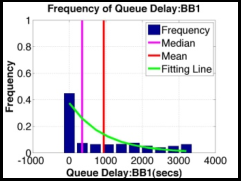
\includegraphics[width=0.4\textwidth]{figures/model/BB1.pdf}
%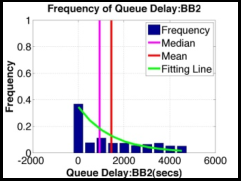
\includegraphics[width=0.4\textwidth]{figures/model/BB2.pdf}
%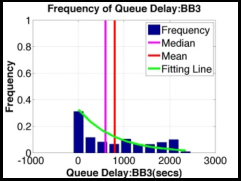
\includegraphics[width=0.4\textwidth]{figures/model/BB3.pdf}
%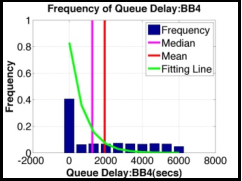
\includegraphics[width=0.4\textwidth]{figures/model/BB4.pdf}
%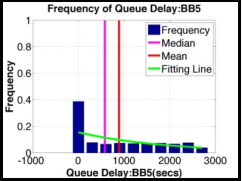
\includegraphics[width=0.4\textwidth]{figures/model/BB5.pdf}
%    \caption{Frequency Distribution of Queue Delay in Broadband}
%    \label{fig:model_broadband_distribution}
%\end{figure}
%
%\begin{table}[h!]
%\caption{Makespan of Broadband}
%\label{tab:model_broadband}
%\centering
%\begin{tabular}{lrrrr}
%\hline
%     &      Makespan &     Num of Nodes &    File System  \\
%\hline
%BB1 & 1:08:17 & 8 & NFS\\
%BB2 & 1:29:23 & 4 & NFS \\
%BB3 & 1:32:57 & 4 & PVFS \\
%BB4 & 1:51:14 & 1 & NFS \\
%BB5 & 0:52:48 & 1 & shm \\
%\hline
%\end{tabular}
%\end{table} 
%
%\begin{table}[h!]
%\caption{the SSE (sum of squares of error) of different fitting distribution}
%\label{tab:model_broadband_sse}
%\centering
%\begin{tabular}{lrrrr}
%\hline
%SSE(Unit: $10^4$)     &      Exponential &  Gamma & Normal & Weibull \\
%\hline
%BB1 & 3.57 & 232 & 8.69 & 235.2\\
%BB2 & 2.33 & 244 & 5.59 & 181.0\\
%BB3 & 1.97 & 73.9 & 4.18 & 52.4\\
%BB4 & 3.31 & 340 & 7.22 & 251.7\\
%BB5 & 2.84 & 73.1 & 6.48 & 55.4 \\
%\hline
%\end{tabular}
%\end{table} 
%
%\begin{table}[h!]
%\caption{the $\mu$ of the exponential fitting distribution}
%\label{tab:model_broadband_mu}
%\centering
%\begin{tabular}{lrrrr}
%\hline
%(Unit: sec)     &      $\mu$ \\
%\hline
%BB1 & 944.85\\
%BB2 & 1451.88\\
%BB3 & 796.90\\
%BB4 & 1952.71\\
%BB5 & 892.16 \\
%\hline
%\end{tabular}
%\end{table} 
%
%\begin{table}[h!]
%\caption{the log likelihood of different fitting distribution}
%\label{tab:model_broadband_log}
%\centering
%\begin{tabular}{lrrrr}
%\hline
%Log Likelihood     &      Exponential &  Gamma & Normal & Weibull \\
%\hline
%BB1 & -6045.3 & -5802.3 & -6464.1 & -5819.6\\
%BB2 & -6376.1 & -6203.1 & -6707.9 & -6232.9\\
%BB3 & -5914.2 & -5796.4 & -6181.4 & -5825.9\\
%BB4 & -6376.1 & -6203.1 & -6707.9 & -6232.9\\
%BB5 & -6001.1 & -5891.9 & -6327.9 & -5908.1 \\
%\hline
%\end{tabular}
%\end{table} 
%
%Frequency distribution analysis serves as an important supplement to the understanding of how different execution environments influence the overheads. Figure~\ref{fig:model_broadband_distribution} presents the mean, median and the exponential fitting lines of Queue Delay in Broadband of five runs (BB1$\sim$BB5). The Broadband workflows were executed in environments with different number of worker nodes and file systems. These runs had the same jobs and used the same type of virtual machines (c1.xlarge), but they were run in different environments. The number of worker nodes was ranging from 1 to 8 and the file systems included NFS \cite{Sandberg1985}, PVFS \cite{Carns2000} and a shared memory system (shm) on a single host. 
%
%Comparing BB1, BB2 and BB4 we conclude that resource availability influences the distribution of the queue delay. Although for all the five runs, most of the queue delays (30\%$\sim$40\%) last less than 50 seconds, the maximum duration of queue delay increases with the decrease of resource availability. With more resources available, the local scheduler is able to find a resource for execution more quickly. BB3 is installed with PVFS, which performs worse than BB2 with NFS in this experiment. The shared memory system can also improve the performance, but it is limited to the case with only one host.  
%
%We use the Matlab Distribution Fitting tool \cite{Matlab} to analyze the distribution of the queue delay. This tool aims to maximize the log likelihood of the parameters. Table~\ref{tab:model_broadband_log} shows that the queue delay satisfies the Weibull and Gamma distribution better in terms of the log likelihood. However, Table~\ref{tab:model_broadband_sse} shows that in terms of SSE (sum of squares of error), the exponential and normal distributions perform better. For simplicity, we use an exponential distribution to describe the queue delay:
%
%\begin{equation} \label{eq:model_f1}
% \phi_1(x)=\frac{1}{\mu}e^{-\frac{x}{\mu}}\varepsilon(x)
%\end{equation}
%
%$\varepsilon(x)$ is an unit step function. The estimates of $\mu$ are listed in Table~\ref{tab:model_broadband_mu}. 

%Figure~\ref{fig:model_cybershake_distribution} shows the mean and standard deviation of all 78 partitions of the entire CyberShake workflow. The standard deviation is comparable to the mean of the overheads, which we attribute to the fact that HPCC comprises a diverse mix of computing and data resources and is shared among many users across the campus. 
Figure~\ref{fig:model_montage_distribution} shows the overhead distribution of the Montage workflow run on the FutureGrid. The postscript delay concentrates at 7 seconds, because the postscript is only used to locally check the return status of a job and is not influenced by the remote execution environment. The workflow engine delay tends to have a uniform distribution, which is because the workflow engine spends a constant amount of time to identify that the parent jobs have completed and insert a job that is ready at the end of the local queue. 
%Normally, the queue delay has only one peak such as in Figure~\ref{fig:model_broadband_distribution}. But in this experiment, 
The queue delay has three decreasing peak points at 8, 14, and 22 seconds. We believe this is because the average postscript delay is about 7 seconds (see details in Figure~\ref{fig:model_montage_distribution} ) and the average runtime is 1 second. The local scheduler spends about 8 seconds finding an available resource and executing a job; if there is no resource idle, it will wait another 8 seconds for the current running jobs to finish, and so on. 
%Based on Equation~\ref{eq:model_f1}, an integrated function of the queue delay can be expressed as a combination of multiple exponential distributions:
%\begin{equation} \label{eq:model_f2}
% \phi_2(x)=\sum_{i=1}^{\infty}e^{-ai}\phi_1(x-ib)
%\end{equation}
%$a$ is the attenuation coefficient of the exponential distribution and $b$ is the average distance between the peaks, namely the period. In the example of Figure~\ref{fig:model_montage_distribution}, $a\approx0.5, b\approx7$. 

%\begin{figure}[h!]
%	\centering
%    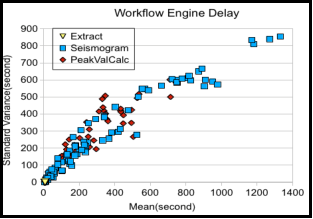
\includegraphics[height=0.3\textwidth]{figures/model/cybershake_engine_delay.pdf}
%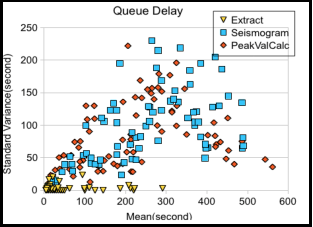
\includegraphics[height=0.3\textwidth]{figures/model/cybershake_queue_delay.pdf}
%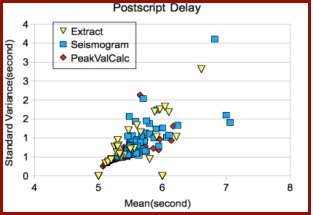
\includegraphics[width=0.4\textwidth]{figures/model/cybershake_post_delay.pdf}
%
%    \caption{Mean and Variance of all the 78 partitions of the CyberShake workflow}
%    \label{fig:model_cybershake_distribution}
%\end{figure}

\begin{figure}[h!]
	\centering
    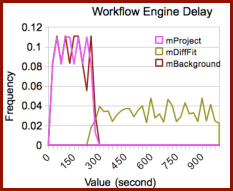
\includegraphics[height=0.3\textwidth]{figures/model/montage_engine_delay.pdf}
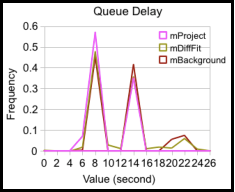
\includegraphics[height=0.3\textwidth]{figures/model/montage_queue_delay.pdf}
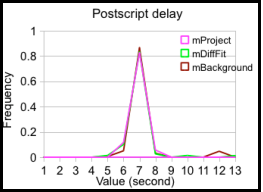
\includegraphics[width=0.4\textwidth]{figures/model/montage_post_delay.pdf}

    \caption{Distribution of overheads in the Montage workflow}
    \label{fig:model_montage_distribution}
\end{figure}

%In our prior work \cite{Overhead2011}, we have introduced the distribution of overheads and the relationship between them. Following this, we indicate the necessity to consider the distribution of overheads rather than simply adding a constant delay after job execution. 
We use Workflow Engine Delay as an example to show the necessity to model overheads appropriately. Figure~\ref{fig:model_montage_timeline} shows a real trace of overheads and runtime in the Montage 8 degree workflow (for visibility issues, we only show the first 15 jobs at the mProjectPP level). We can see that Workflow Engine Delay increases steadily after every five jobs. For example, the Workflow Engine Delay of jobs with ID from 6 to 10 is approximately twice of that of jobs ranging from ID1 to ID5. Figure~\ref{fig:model_montage_five_runs} further shows the distribution of Workflow Engine Delay at the mProjectPP level in the Montage workflow that was run five times. After every five jobs, the Workflow Engine Delay increases by 8 seconds approximately. We call this special nature of workflow overhead as cyclic increase. The reason is that Workflow Engine (in this trace it is DAGMan) releases five jobs by default in every working cycle. Therefore, simply adding a constant delay after every job execution has ignored its potential influence on the performance.

\begin{figure}[h!]
	\centering
    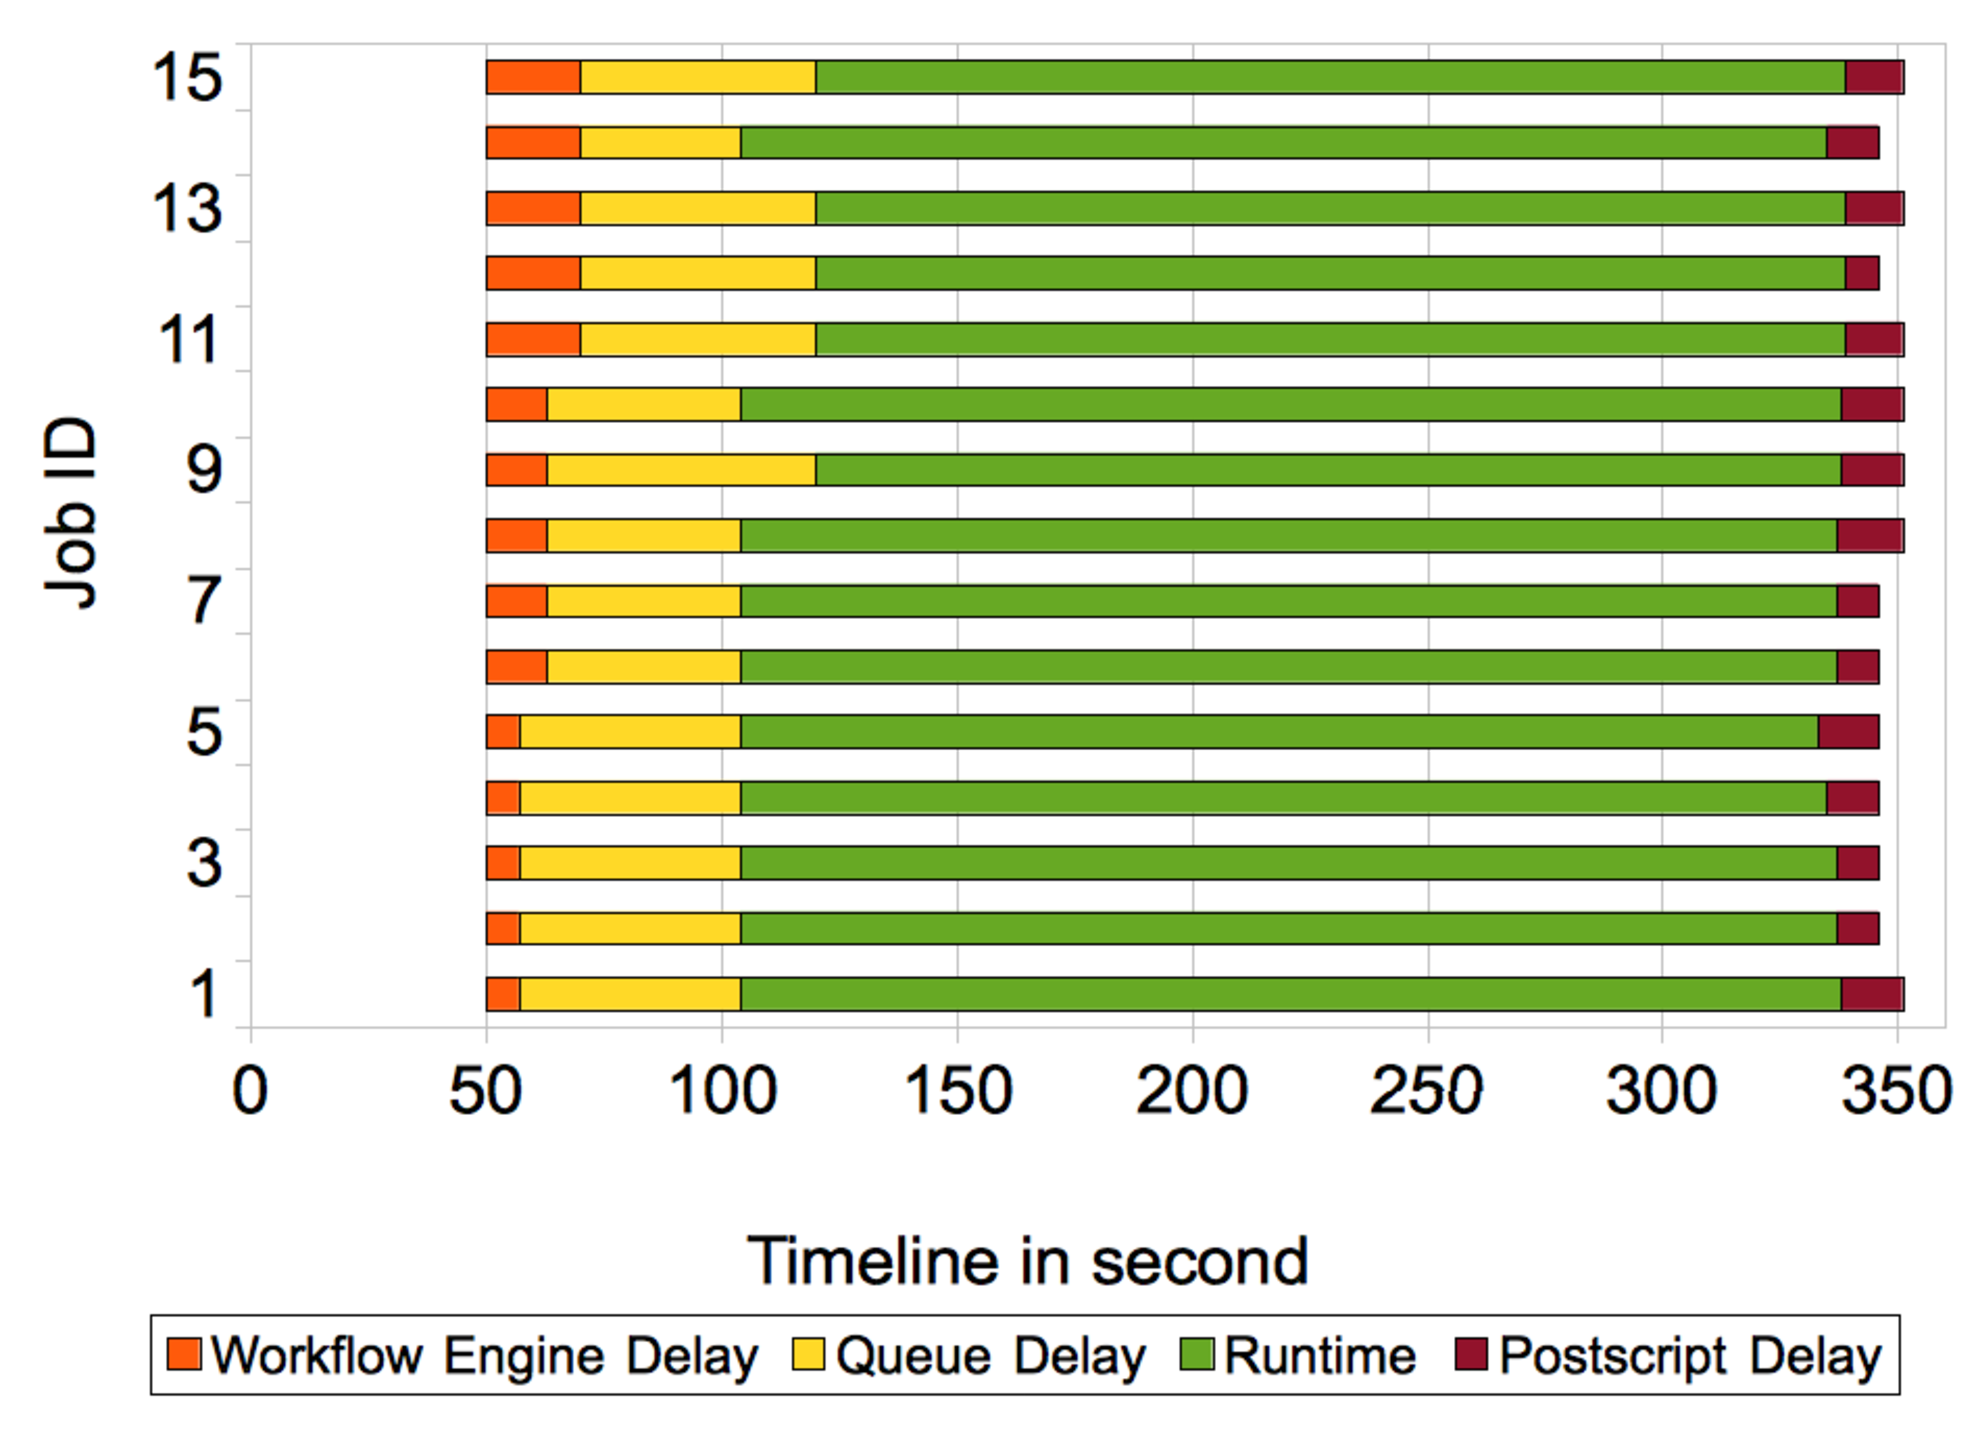
\includegraphics[width=0.7\textwidth]{figures/model/overhead_timeline2.pdf}
    \caption{Workflow Overhead and Runtime. Clustering delay and data transfer delay are not shown}
    \label{fig:model_montage_timeline}
\end{figure}




\begin{figure}

\centering
  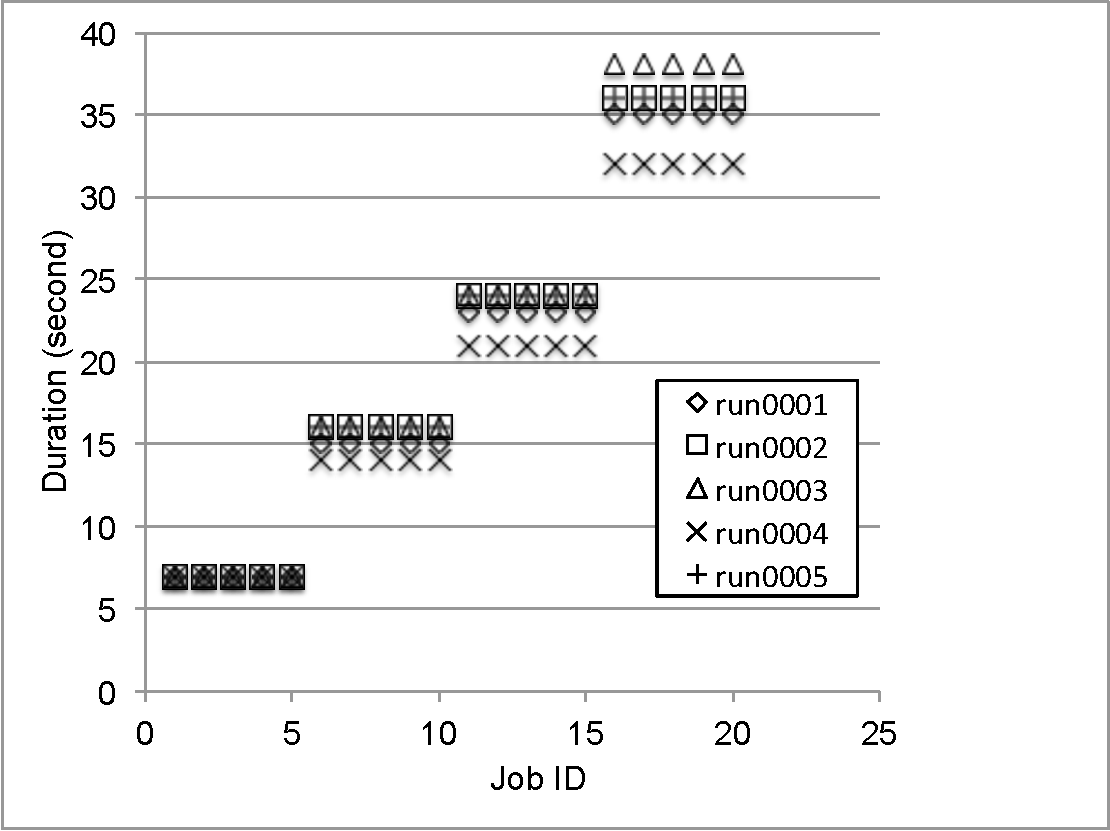
\includegraphics[width=0.6\linewidth]{figures/model/montage_five_runs.pdf}
    \caption{Workflow Engine Delay of mProjectPP}
    \label{fig:model_montage_five_runs}
\end{figure}%
\begin{figure}
  \centering
  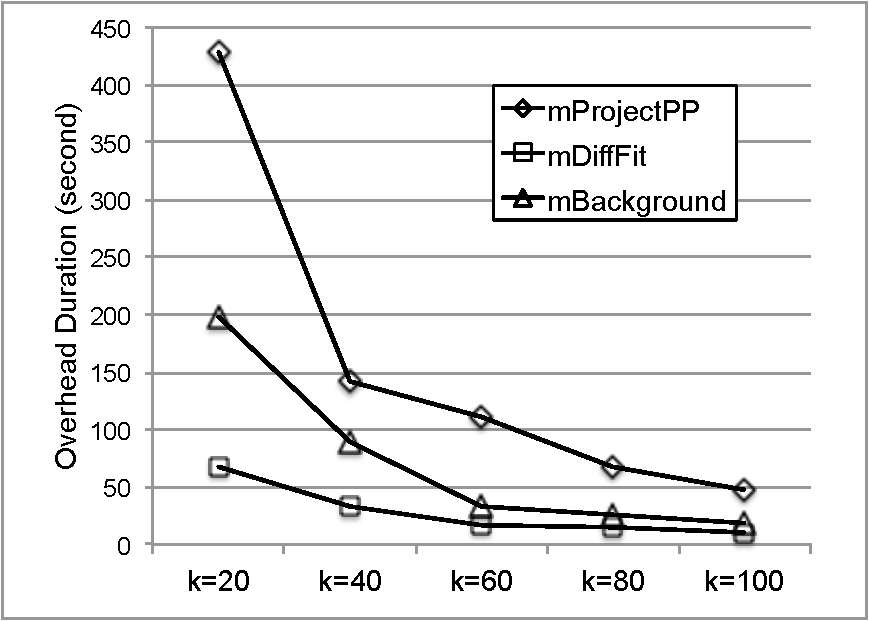
\includegraphics[width=0.6\linewidth]{figures/model/montage_clustering_delay.pdf}
    \caption{Clustering Delay of mProjectPP, mDiffFit, and mBackground}
    \label{fig:model_montage_clustering}
\end{figure}





Figure~\ref{fig:model_montage_clustering} shows the average value of Clustering Delay of mProjectPP, mDiffFit, and mBackground. It is clear that with the increase of $k$ (the maximum number of jobs per horizontal level), since there are less and less tasks in a clustered job, the Clustering Delay for each job decreases. For simplicity, we use an inverse proportional model in Equation~\ref{eq:model_clustering_delay} to describe this trend of Clustering Delay with $k$. Intuitively we assume that the average delay per task in a clustered job is constant ($n$ is the number of tasks in a horizontal level). An inverse proportional model can estimate the delay when $k=i$ directly if we have known the delay when $k=j$. Therefore we can predict all the clustering cases as long as we have gathered one clustering case. 

\begin{equation} \label{eq:model_clustering_delay}
\frac{Clustering Delay|_{k=i}}{Clustering Delay|_{k=j}}=\frac{n/i}{n/j}=\frac{j}{i}
\end{equation}



\subsection{Metrics to Evaluate Cumulative Overheads}

After identifying the major overheads in workflows and describe how they are measured based on workflow events, we provide an integrated and comprehensive quantitative analysis of workflow overheads. The observation on overhead distribution and characteristics enable researchers to build a more realistic model for simulations of real applications. Our analysis also offers guidelines for developing further optimization methods. 

%We propose several metrics to calculate the cumulative sum of the overheads based on how they overlap and their importance in the graph. In addition, we indicate how experimental parameters impact the overhead and thereby the overall workflow performance. We then show how popular optimization methods improve runtime performance by reducing some or all types of overheads. 

In this section, we define four metrics to calculate cumulative overheads of workflows, which are $Sum$, $Projection(PJ)$, $Exclusive~Projection(EP)$ and $Reverse~Ranking(RR)$. $Sum$ simply adds up the overheads of all jobs without considering their overlap. $PJ$ subtracts from $Sum$ all overlaps of the same type of overhead. It is equal to the projection of all overheads to the timeline. $EP$ subtracts the overlap of all types of overheads from $PJ$. It is equal to the projection of overheads of a particular type excluding all other types of overheads to the timeline.
$RR$ uses a reverse ranking algorithm to index overheads and then calculates the cumulative overhead weighted by the ranks. The idea is brought by web page indexing algorithms such as PageRank \cite{PageRank1999}. Figure~\ref{fig:model_rr} shows how to calculate the reverse ranking value $(RR)$ of the same workflow graph in Figure~\ref{fig:model_overhead_timeline}.
 
\begin{equation} \label{eq:model_rr}
RR(j_u)=d+(1-d)\times\sum_{j_v\in Child(j_u)}{}\frac{RR(j_v)}{L(j_v)}
\end{equation}

Equation~\ref{eq:model_rr} means that the $RR$ of a node (overhead or job) is determined by the $RR$ of its child nodes. $d$ is the damping factor, which usually is 0.15 as in PageRank. $L(j_v)$ is the number of parents that node $j_v$ has. Intuitively speaking, a node is more important if it has more child nodes and its child nodes are more important. In terms of workflows, it means an overhead has more power to control the release of other overheads and computational activities. There are two differences compared to the original PageRank: 
\begin{enumerate}
\item We use output link pointing to child nodes while PageRank uses input link from parent nodes, which is why we call it reverse ranking algorithm.
\item Since a workflow is a DAG, we do not need to calculate $RR$ iteratively. For simplicity, we assign the $RR$ of the root node to be 1. And then we calculate the $RR$ of a workflow ($G$) based on the equation below:

\begin{equation} \label{eq:model_sum_rr}
RR(G)=\sum_{}{}RR(j_u) \times \phi_{j_u}
\end{equation}

\end{enumerate}
 
$\phi_{j_u}$ indicates the duration of job $j_u$.  $RR$ evaluates the importance of an overhead and represents the cumulative overhead weighted by this importance. 
The reason we have four metrics of calculating cumulative overheads is to present a comprehensive overview of the impact of overlaps between the various overheads and runtime. Many optimization methods such as Data Placement Services \cite{Amer2012} try to overlap overheads and runtime to improve the overall performance. By analyzing these four types of cumulative overheads, researchers have a clearer view of whether their optimization methods have overlapped the overheads of a same type (if $PJ < Sum$) or other types (if $EP < PJ$). $RR$ shows the connectivity within the workflow, the larger the denser. 
We use a simple example workflow with three jobs to show how to calculate the overlap and cumulative overheads. Figure~\ref{fig:model_overhead_timeline} shows the timeline of our example workflow. Job1 is a parent job of Job 2 and Job 3.

\begin{figure}[h!]
	\centering
    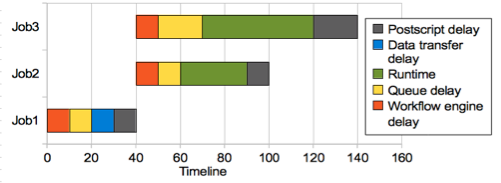
\includegraphics[width=0.6\textwidth]{figures/model/overhead_timeline.pdf}
    \caption{The Timeline of an Example Workflow}
    \label{fig:model_overhead_timeline}
\end{figure}
\begin{figure}[h!]
	\centering
    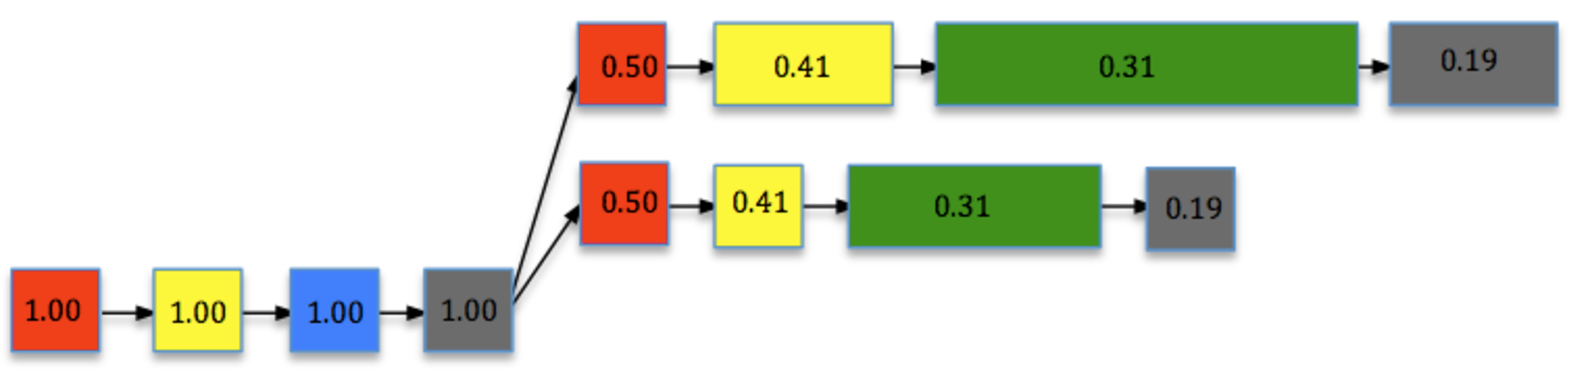
\includegraphics[width=0.7\textwidth]{figures/model/rr.pdf}
    \caption{Reverse Ranking}
    \label{fig:model_rr}
\end{figure}
At $t=0$, job 1, a stage-in job, is released: $queue~delay = 10$, $workflow~engine~delay = 10$, $runtime = 10$, and $postscript~delay = 10$.
At $t=40$, job 3 is released: $workflow~engine~delay = 10$, $queue~delay = 20$, $runtime = 50$, and $postscript~delay = 20$.
At $t=40$, job 2 is released: $workflow~engine~delay = 10$, $queue~delay = 10$, $runtime = 30$, $postscript~delay = 10$. 

%We show how to calculate the cumulative overheads:
 
%For $Sum$:
%$Sum(runtime)=50+30=80$. It contains the time slots of [60, 90] and [70, 120]. 
%$Sum(queue~delay)=10+20+10=40$. It contains [10, 20], [50, 70] and [50, 60]. 
%$Sum(workflow~engine~delay)=10+10+10=30$. It contains [0,10], [40, 50] and [40, 50]. 
%$Sum(postscript~delay)=10+20+10=40$. It contains [30, 40], [90, 100] and [120, 140]. 
%$Sum(data~transfer~delay)=10$. It contains [20, 30].

%For $PJ$:
%$PJ(runtime)=50+30-20=60$. It contains [60, 120].
%$PJ(queue~delay)=10+20+10-10=30$. It contains [10, 20] and [50, 70].
%$PJ(workflow~engine~delay)=10+10+10-10=20$. It contains [0, 10] and [40, 50].
%$PJ(postscript~delay)=10+20+10=40$. It contains [30, 40], [90, 100] and [120, 140].
%$PJ(data~transfer~delay)=10$. It contains [20, 30].

%For $EP$: 
%$EP(runtime)=50+30-20-10-10=40$. It contains [70, 90] and [100, 120].
%$EP(queue~delay)=10+20+10-10-10=20$. It contains [10, 20] and [50, 60]. 
%$EP(workflow~engine~delay)=10+10+10-10=20$. It contains [0, 10] and [40, 50]. 
%$EP(postscript~delay)=10+20+10-10=30$. It contains [30, 40] and  [120,140]. 
%$EP(data~transfer~delay)=10$. It contains [20, 30].

%$RR(runtime)=50\times 0.31+30\times 0.31=24.8$.
%$RR(queue~delay)=10\times 1.00+10\times 0.41+10\times 0.41=18.2$.
%$RR(workflow~engine~delay)=10\times 1.00+10\times 0.50+10\times 0.50=20$.
%$RR(postscript~delay)=10\times 1.00+10\times 0.19+20\times 0.19=15.7$.
%$RR(data~transfer~delay)=10\times 1.00=10$.

In calculating the cumulative runtime, we do not include the runtime of stage-in jobs because we have already classified it as data transfer delay. The overall makespan for this example workflow is 140. Table~\ref{tab:model_percentage_overhead} shows the percentage of overheads and job runtime over makespan.  

\begin{table}[h!]
\caption{Percentage of Overheads and Runtime}
\label{tab:model_percentage_overhead}
\centering
\begin{tabular}{lrrrr}
\hline
Percentage & Sum & PJ & EP &RR\\

\hline

runtime & 57.14\% & 42.86\% & 28.57\% &17.71\% \\
queue delay & 28.57\% &21.43\% &14.29\% &13.00\% \\
workflow engine delay & 21.43\% &14.29\%& 14.29\% &14.29\%\\
postscript delay & 28.57\% & 28.57\% & 21.43\% & 11.21\% \\
data transfer delay & 7.14\% & 7.14\% & 7.14\% & 7.14\% \\
sum & 142.86\% & 114.29\% & 85.71\% & 63.36\%\\
\hline
\end{tabular}
\end{table} 


In Table~\ref{tab:model_percentage_overhead}, we can conclude that the sum of $Sum$ is larger than makespan and smaller than makespan$\times$(number of resources) because it does not count the overlap at all. $PJ$ is larger than makespan since the overlap between more than two types of overheads may be counted twice or more. $EP$ is smaller than makespan since some overlap between more than two types of overheads may not be counted.  $RR$ shows how intensively these overheads and computational activities are connected to each other. 

%Should be included in final defense
%\subsection{Relationship between Overhead Metrics and Overall Performance}

%In this section, we aim to investigate the relationship between the overhead metrics that we proposed and the overall performance of popular workflow restructuring techniques. Among them, task clustering \cite{Singh2008} is a technique that increases the computational granularity of tasks by merging small tasks together into a clustered job, reducing the impact of the queue wait time and also the makespan of the workflow. Data or job throttling \cite{Humphrey2008} limits the amount of parallel data transfer to avoid overloading supporting services such as data servers. Throttling is especially useful for unbalanced workflows in which one task might be idle while waiting for data to arrive. The aim of throttling is to appropriately regulate the rate of data transfers between the workflow tasks via data transfer servers by ways of restricting the data connections, data threads or data transfer jobs. Provisioning tools often deploy pilot jobs as placeholders for the execution of application jobs. Since a placeholder can allow multiple application jobs to execute during its lifetime, some job scheduling overheads can be reduced. 

%\textbf{How Task Clustering Reduces Overheads}

%In the following sections, we use a Montage workflow to show how different optimization methods improve overall performance. Many workflows are composed of thousands of fine computational granularity tasks. Task clustering is a technique that increases the computational granularity of tasks by merging small jobs together into a clustered job, reducing the impact of the queue wait time and minimizing the makespan of the workflow. Table 4.2 compares the overheads and runtime of the Montage workflow. We can conclude that with clustering, although the average overheads do not change much, the cumulative overheads decrease greatly due to the decreased number of jobs. With clustering, the makespan has been reduced by 53.3\% by reducing the number of all jobs from 3461 to 104 in this example. Figure 4.5 shows the percentage of workflow overheads and runtime. The percentage is calculated by the cumulative overhead ($PJ$, or $EP$) divided by the makespan of workflows. With clustering, the portion of runtime is increased significantly. Figure 4.6 profiles the number of active jobs during execution and it also shows that with clustering the resource utilization is improved significantly. 

%\textbf{How Job Throttling Reduces Overheads}

%Data or job throttling [13] limits the amount of parallel data transfer to avoid overloading supporting services such as data servers. Throttling is especially useful for unbalanced workflows in which one task might be idle while waiting for data to arrive. The aim of throttling is to appropriately regulate the rate of data transfers between the workflow tasks via data transfer servers by ways of restricting the data connections, data threads or data transfer jobs. Especially on cloud platforms, I/O requests need to go through more layers than a physical cluster; and thereby workflows may suffer a higher overhead from data servers.

%In our experiments, the data transfer service is deployed on a virtual machine that is similar to a worker node.  In this section, we evaluate a simple static throttling strategy where the Condor scheduler limits the number of concurrent jobs to be run and thereby restricts the number of parallel I/O requests. There are 32 resources available and we evaluate the cases with throttling parameters that are equal to 24, 16 and 12 in Table 4.3. In the case of 24, the resources are better utilized but the data server is heavily loaded. In the case of 12, the resources are under-utilized even though the data server has more capabilities. In this experiment, both $PJ$ and $EP$ reflect the variation trend of overheads and makespan better than $Sum$. 

%Figure 4.7 shows the percentage of workflow overheads and runtime. Figure 4.8 profiles the number of active jobs during execution. Montage is an unbalanced workflow because the three major types of jobs (mProjectPP, mDiffFit, and mBackground) impose a heavy load on the data server while the other jobs in the workflow do not. Figure 4.8 shows that with throttling the maximum number of active jobs is restricted. With limited throttling (reducing threshold from 24 to 16), the data transfer requests are distributed in the timeline more evenly and, as a result, their overhead is reduced. However, with over throttling (reducing threshold from 16 to 12), resources are not fully utilized and thus the makespan is increased. 

%\textbf{How Pre-staging Reduces Overheads}

%Scientific workflows often consume and produce a large amount of data during execution. Data pre-staging [14] transfers input data before the computational activities are started or even before the workflow is mapped onto resources. Data placement policies distribute data in advance by placing data sets where they may be requested or by replicating data sets to improve runtime performance. In our experiments, because data is already pre-staged, the implementation of the stage-in job is to create a soft link to the data from the workflow’s working directory, making it available to the workflow jobs. Table 4.4 and Figure 4.9 show the cumulative overheads and runtime of the Montage workflows running with and without pre-staging. Looking at the rows for $PJ$ in Table 4.4, we can conclude that pre-staging improves the overall runtime by reducing the data transfer delay. For the case without pre-staging the $EP$ for data transfer delay is zero because it overlaps with the workflow engine delay of another job. Therefore, in this experiment, $PJ$ reflects the variation trend of the makespan more consistently. 

%\textbf{How Provisioning Reduces Overheads}

%Many of the scientific applications presented here consist of a large number of short-duration tasks whose runtimes are greatly influenced by overheads present in distributed environments. Most of these environments have an execution mode based on batch scheduling where jobs are held in a queue until resources become available to execute them. Such a best-effort model normally imposes heavy overheads in scheduling and queuing. For example, Condor-G [23] uses Globus GRAM [37] to submit jobs to remote clusters. The Globus Toolkit normally has a significant overhead compared to running Condor directly as an intra domain resource and job management system. Provisioning tools often deploy pilot jobs as placeholders for the execution of application jobs. Since a placeholder can allow multiple application jobs to execute during its lifetime, some job scheduling overheads can be reduced. In our experiments, we compared the performance of Condor-G (without provisioning) and Corral (with provisioning). 

%Table 4.5 and Figure 4.10 show the percentage of workflow overheads and runtime. The percentage is calculated by the cumulative overhead ($Sum$, $PJ$, or $EP$) divided by the makespan of workflows. Comparing $Sum$, $PJ$ and $EP$, we can conclude that the overheads with provisioning have been reduced significantly because the local scheduler has direct control over the resources without going through Globus. 

\section{Experiments and Discussion}

In this section, we introduce our workflow simulator called WorkflowSim that utilizes the o-DAG model to simulate large scale workflows. We verify its effectiveness through a series of experiments. The evaluation of the performance of workflow optimization techniques in real infrastructures is complex and time consuming. As a result, simulation-based studies have become a widely accepted way to evaluate workflow systems. For example, scheduling algorithms, such as HEFT \cite{Topcuoglu2002}, MaxMin \cite{Braun2001}, MinMin \cite{Blythe2005}, etc., have used simulators to evaluate their effectiveness. A simulation-based approach reduces the complexity of the experimental setup and saves much effort in workflow execution by enabling the testing of their applications in a repeatable and controlled environment. 


\begin{figure}[h!]
	\centering
    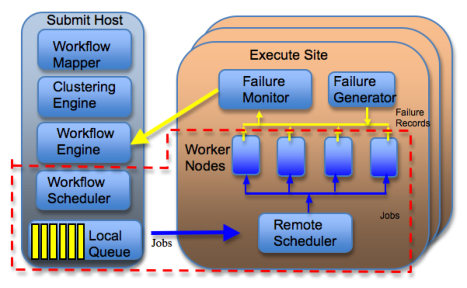
\includegraphics[width=0.7\textwidth]{figures/model/wfs_overview.pdf}
    \caption{WorkflowSim Overview. The area surrounded by red lines is supported by CloudSim}
    \label{fig:model_wfs_overview}
\end{figure}

However, an accurate simulation framework for scientific workflows is required to generate reasonable results, particularly considering that the overall system overhead \cite{Overhead2011} plays a significant role in the workflow’s runtime. 
%In heterogeneous distributed systems, workflows may experience different types of overheads, which are defined as the time of performing miscellaneous work other than executing users’ computational activities.  Since the causes of overheads differ, the overheads have diverse distributions and behaviors. For example, the time to run a post-script that checks the return status of a computation is usually a constant. However, queue delays incurred while tasks are waiting in a batch scheduling systems can vary widely. 
By classifying these workflow overheads in different layers and system components, our simulator can offer a more accurate result than simulators that do not include overheads in their system models.

What’s more, many researchers \cite{Zhang2004, Tang1990, Schroeder2006, Sahoo2004, Oppenheimer2002, Mcconnel} have emphasized the importance of fault tolerant design and concluded that the failure rates in modern distributed systems should not be neglected. A simulation with support for randomization and layered failures is supported in WorkflowSim to promote such studies. 

Finally, progress in workflow research also requires a general-purpose framework that can support widely accepted features of workflows and optimization techniques. Existing simulators such as CloudSim/GridSim \cite{Calheiros2011} fail to provide fine granularity simulations of workflows. For example, they lack the support of task clustering, which is a popular technique that merges small tasks into a large job to reduce task execution overheads. The simulation of task clustering requires two layers of execution model, on both task and job levels. It also requires a workflow-clustering engine that launches algorithms and heuristics to cluster tasks. Other techniques such as workflow partitioning and task retry are also ignored in these simulators. These features have been implemented in WorkflowSim. 

%To the best of our knowledge, none of the current distributed system simulators support these rich-features and techniques. In this section, we introduce our early work on simulating scientific workflows satisfying these requirements. We evaluate the performance of WorkflowSim with an example of task clustering. We further show that WorkflowSim is promising in providing an evaluation platform for research areas such as fault tolerant clustering and overhead robustness studies. 

\subsection{Components of WorkflowSim}

As Fig~\ref{fig:model_wfs_overview} shows, there are multiple layers of components involved in preparing and executing a workflow. Among them, Workflow Mapper, Workflow Engine, Workflow Scheduler and Job Execution have been introduced in last section. Below we introduce three components that have not been introduced. 
\begin{enumerate}

\item Clustering Engine

The Clustering Engine merges tasks into jobs so as to reduce the scheduling overheads. 

%\item Workflow Engine 

%The Workflow Engine manages jobs based on their dependencies to assure that a job may only be released when all of its parent jobs have completed successfully. The Workflow Engine will only release free jobs to the Scheduler. In the real execution we studied, we use DAGMan \cite{DAGMan} as the Workflow Engine. 
  
%\item Workflow Scheduler and Job Execution

%The Workflow Scheduler is used to match jobs to worker nodes based on the criteria selected by users (MaxMin \cite{Braun2001}, MinMin \cite{Blythe2005} , and many other heuristics). While CloudSim has already supported static scheduling algorithms, we added the support of dynamic workflow algorithms. For static algorithms, jobs are assigned to a worker node at the workflow planning stage. When the job reaches the remote scheduler, it will just wait until the assigned worker node is free. For dynamic algorithms, jobs are matched to a worker node in the remote scheduler whenever a worker node becomes idle. WorkflowSim relies on CloudSim to provide an accurate and reliable job-level execution model, such as time-shared model and space-shared model. However, WorkflowSim has introduced different layers of overheads and failures, which improves the accuracy of simulation. 

%\begin{figure}[h!]
%	\centering
 %   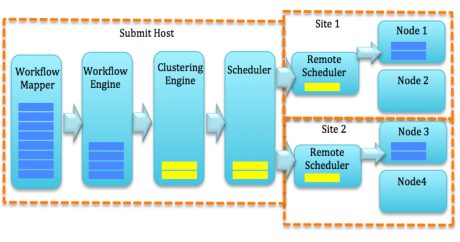
\includegraphics[width=0.7\textwidth]{figures/model/wfs_interaction.pdf}
  %  \caption{Interaction between components}
   % \label{fig:model_wfs_interaction}
%\end{figure}


%To associate and coordinate these layers, we adopted an event-based approach where each component maintains a message queue. Fig~\ref{fig:model_wfs_interaction} shows a simple configuration with two execution sites, of which each has two nodes. Each component maintains its own message queue and iteratively checks whether it can process one message. For example, at each iteration, the Clustering Engine checks whether it has received new tasks from the Workflow Engine and whether it should release new jobs to the Scheduler. When none of these components have any more messages in queue, the simulation is completed. 

%Based on our prior studies on workflow overheads, we add layered overhead to the workflow simulation. We have classified workflow overheads into five categories as follows. 
%\begin{enumerate}

%\item Workflow Engine Delay measures the time between when the last parent job of a job completes and the time when the job gets submitted to the local queue. In case of retries the value of the last retry is used for the calculation. Since we use a DAG model to represent workflows, the completion time of the last parent job means this job is released to the ready queue and is waiting for resources to be assigned to it. The workflow engine delay reflects the efficiency of a workflow engine (in our case DAGMan). 

%\item Queue Delay is defined as the time between the submission of a job by the workflow engine to the local queue and the time the local scheduler sees the job running (potentially on remote resources). This overhead reflects the efficiency of the workflow scheduler (e.g., Condor \cite{Frey2002}) to execute a job and the availability of resources for the execution of the job. In case of retries the value is the cumulative of all the retries.  
%\item Postscript Delay and Prescript Delay is the time taken to execute a lightweight script under some execution systems before and after the execution of a job. Prescripts are usually used to create directories for job execution. Postscripts examine the exit code of a job after the computational part of the job is done.
%\item Data Transfer Delay happens when data is transferred between nodes. It includes three different types of processes: staging data in, cleaning up, and staging data out. Stage-in jobs transfer input files from source sites to execution sites before the computation starts. Cleanup jobs delete intermediate data that is no longer needed by the remainder of the workflow. Stage-out jobs transfer workflow output data to archiving sites for storage and analysis.
%\item Clustering Delay measures the difference between the sum of the actual task runtime and the job runtime seen by the Workflow Scheduler. The cause of Clustering Delay is usually the use a job wrapper used to execute a clustered job. The wrapper takes some time to extract the list of tasks and to launch them. 
%\end{enumerate}                        

%Failures can occur at different times during the workflow execution. Consistent with the definition of tasks and job, we divide transient failures into two categories: task failure and job failure. If the transient failure affects the computation of a task (task failure), other tasks within the job do not necessarily fail. If the transient failure affects the clustered job (job failure), all of its tasks fail. We have added two components in response to the simulation of failures:
\item Failure Generator component is introduced to inject task/job failures at each execution site. After the execution of each job, Failure Generator randomly generates task/job failures based on the distribution and average failure rate that a user has specified. 
\item Failure Monitor collects failure records (e.g., resource id, job id, task id) and returns them to the workflow management system so that it can adjust the scheduling strategies dynamically. 
\end{enumerate}
We also modified other components to support fault tolerant optimization. In a failure-prone environment, there are several options to improve workflow performance. First, one can simply retry the entire job or only the failed part of this job when its computation is not successful. This functionality is added to the Workflow Scheduler, which checks the status of a job and takes action based on the strategies that a user selects. Furthermore, Reclustering is a technique that we have proposed \cite{Chen2012} that aims to adjust the task clustering strategy based on the detected failure rate. This functionality is added to the Workflow Engine. 

\subsection{Experiments and Validation}
We use task clustering as an example to illustrate the necessity of introducing overheads into workflow simulation. The goal was to compare the simulated overall runtime of workflows in case the information of job runtime and system overheads are known and extracted from prior traces. 
In this example, we collected real traces generated by the Pegasus Workflow Management System while executing workflows on FutureGrid \cite{FutureGrid}. We built an execution site with 20 worker nodes and we executed the Montage workflow five times in every single configuration of $k$, which is the maximum number of clustered jobs in a horizontal level. These five traces of workflow execution with the same $k$ is a training set or a validation set. 
%Partly illustrated by Figure 5, the results are stable enough to be used as a training set. 
We ran the Montage workflow with a size of 8-degree squares of sky. The workflow has 10,422 tasks and 57GB of overall data. We tried different k from 20 to 100, leaving us 5 groups of data sets with each group having 5 workflow traces. 
First of all, we adopt a simple approach that selects a training set to train WorkflowSim and then use the same training set as validation set to compare the predicted overall runtime and the real overall runtime in the traces. We define accuracy in this section as the ratio between the predicted overall runtime and the real overall runtime:
\begin{equation} \label{eq:model_wfs_accuracy}
Accuracy=\frac{Predicted~Overall~Runtime}{Real~Overall~Runtime}
\end{equation}
 \begin{figure}[h!]
	\centering
    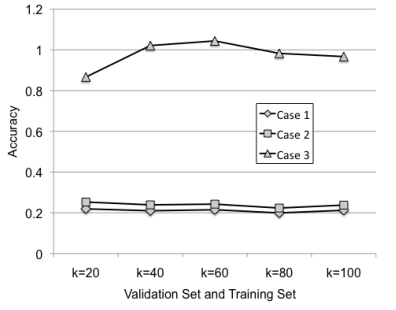
\includegraphics[width=0.6\textwidth]{figures/model/wfs_levels.pdf}
    \caption{Performance of WorkflowSim with different support levels}
    \label{fig:model_wfs_levels}
\end{figure} 
 
Performance of WorkflowSim with different support levels. 
To train WorkflowSim, from the traces of workflow execution (training sets), we extracted information about job runtime and overheads, such as average/distribution and, for example, whether it has a cyclic increase. We then added these parameters into the generation of system overheads and simulated them as close as possible to the real cases. Here, we do not discuss the randomization or distribution of job runtime since we rely on CloudSim to provide a convincing model of job execution.

To present an explicit comparison, we simulated the cases using WorkflowSim that has no consideration of workflow dependencies or overheads (Case 1), WorkflowSim with Workflow Engine that has considered the influence of dependencies but ignored overheads (Case 2), and WorkflowSim, that has covered both aspects (Case 3). Intuitively speaking, we expect that the order of the accuracy of them should be Case 3 $>$ Case 2 $>$ Case 1. 

% \begin{figure}[h!]
%	\centering
%    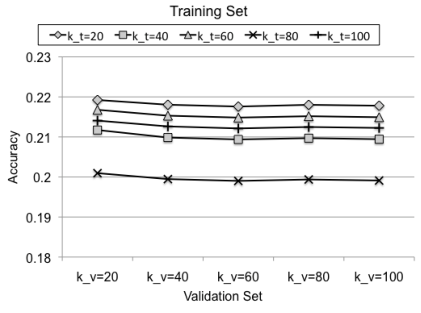
\includegraphics[width=0.6\textwidth]{figures/model/wfs_case1.pdf}
%    \caption{Performance of WorkflowSim of Case 1 (No workflow engine, or overhead support)}
 %   \label{fig:model_wfs_case1}
%\end{figure} 
 
%\begin{figure}[h!]
%	\centering
 %   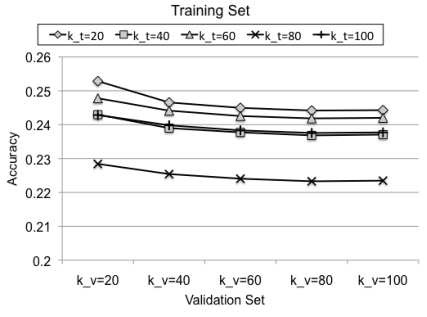
\includegraphics[width=0.6\textwidth]{figures/model/wfs_case2.pdf}
  %  \caption{Performance of WorkflowSim of Case 2 (No overhead support)}
    %\label{fig:model_wfs_case2}
%\end{figure} 

Fig~\ref{fig:model_wfs_levels} shows the performance of WorkflowSim with different support levels is consistent to our expectation. The accuracy of Case 3 is quite close to but not equal to 1.0 in most points. The reason is that to simulate workflows, WorkflowSim has to simplify models with a few parameters, such as the average value and the distribution type. It is not efficient to recur every overhead as is present in the real traces. It is also impossible to do since the traces within the same training set may have much variance. Fig~\ref{fig:model_wfs_levels} also shows that the accuracy of both Case 1 and Case 2 are much lower than Case 3. The reason why Case 1 does not give an exact result is that it ignores both dependencies and multiple layers of overheads. By ignoring data dependencies, it releases tasks that are not supposed to run since their parents have not completed (a real workflow system should never do that) and thereby reducing the overall runtime. At the same time, it executes jobs/tasks irrespective of the actual overheads, which further reduces the simulated overall runtime. In Case 2, with the help of Workflow Engine, WorkflowSim is able to control the release of tasks and thereby the simulated overall runtime is closer to the real traces. However, since it has ignored most overheads, jobs are completed and returned earlier than that in real traces. The low accuracy of Case 1 and Case 2 confirms the necessity of introducing overhead design into our simulator. 

%To further evaluate our task/job model and the performance of WorkflowSim, we adopted a cross-validation approach in which we picked up one group of data set (e.g., $k_t=20$) as input traces/training sets and simulated all the validation sets with $k_v=20$ to 100. To make it clear, we use $k_t$ to indicate the $k$ for a training set and $k_v$ for a validation set. Then we compare the accuracy in Fig~\ref{fig:model_wfs_case1}, Fig~\ref{fig:model_wfs_case2} and Fig~\ref{fig:model_wfs_case3} respectively. 
 
%\begin{figure}[h!]
%	\centering
%    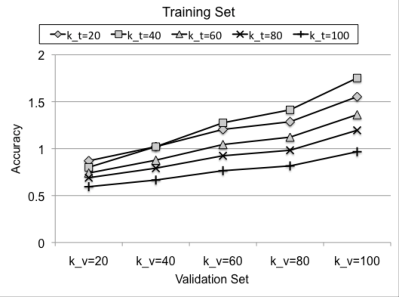
\includegraphics[width=0.6\textwidth]{figures/model/wfs_case3.pdf}
%   \caption{Performance of WorkflowSim of Case 3 (all features are enabled).}
%  \label{fig:model_wfs_case3}
%\end{figure} 

%Fig~\ref{fig:model_wfs_case1} and Fig~\ref{fig:model_wfs_case2} show similar conclusion as in Fig~\ref{fig:model_wfs_levels} and the accuracy of Case 2 and Case 1 are not sensitive to the task clustering. The reason is that Case 1 has no support of data dependencies, where jobs are all submitted at the beginning of workflow execution.  Case 2 has no support of system overhead and thereby task clustering does not improve the overall runtime much. Fig~\ref{fig:model_wfs_case3} shows the simulated results of WorkflowSim, which has considered both layered overhead and data dependencies. Although the accuracy is closer to 1.0, it still does not guarantee a 100\% accuracy in some cases. Particularly when we use a training set with a smaller k (e.g., $k_t=20$) to simulate the case with larger k (e.g., $k_v=100$), the accuracy suffers (accuracy=1.8). The reason is that the average Clustering Delay in the case of $k=20$ is much larger than that of other cases (as shown in Fig~\ref{fig:model_wfs_case2}), and thereby it is still larger than the predicted one using an inverse proportion function. Using such a large Clustering Delay to simulate the case with many clustered jobs ($k_v$ is large) would extend the predicted overall runtime of workflow. Our model has simplified and classified the distribution of overheads based on the horizontal level of tasks but we still need to further study the overhead distribution in accordance to different clustering strategies. However, a complex model may limit its general usage.  

%\subsection{Applications}

%With the features introduced in last section, we are able to carry out research studies such as evaluation of overhead robustness of DAG scheduling heuristics

%\begin{figure}[h!]
%	\centering
%    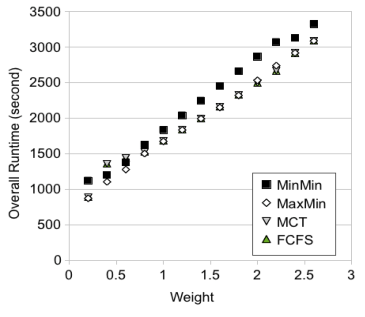
\includegraphics[width=0.6\textwidth]{figures/model/wfs_queue_delay.pdf}
%    \caption{Influence of Queue Delay. The duration of overheads are multiplied by the weights.}
%   \label{fig:model_wfs_queue_delay}
%\end{figure} 

%With the emergence of distributed heterogeneous systems, such as grids and clouds, and applications such as  large scale of workflows with  complex data dependencies, significant overheads can be incurred during workflow execution. Most of the existing DAG scheduling heuristics underestimate or even ignore the influence of workflow overheads. In such a distributed environment, a carefully crafted schedule based on deterministic and static information may fail to provide a sufficient solution. In this study, we analyze the overhead robustness of multiple static and dynamic DAG scheduling heuristics. Overhead robustness describes the influence of overheads on the workflow runtime. We investigate whether the dynamic change in workflow overheads influences the overall runtime of workflows. The reason why we are interested in this study is that in reality, system overheads are difficult to estimate or track. Existing heuristics and algorithms may have different sensitivity to the dynamic change of system overhead or the inaccurate estimation of them. Analyzing their performance in terms of the change of overheads can offer us a unique aspect of their robustness in real systems and suggest the direction of designing new heuristics or algorithms.

%\begin{figure}[h!]
%	\centering
%    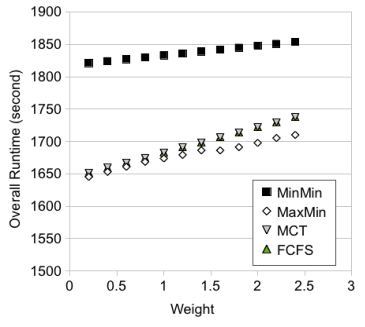
\includegraphics[width=0.6\textwidth]{figures/model/wfs_engine_delay.pdf}
%    \caption{Influence of Workflow Engine Delay}
%    \label{fig:model_wfs_engine_delay}
%\end{figure} 
%\begin{figure}[h!]
%	\centering
%    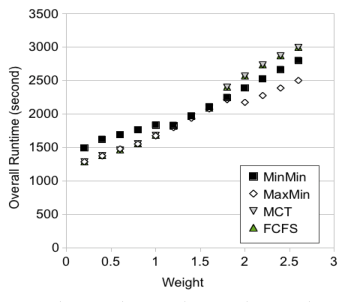
\includegraphics[width=0.6\textwidth]{figures/model/wfs_clustering_delay.pdf}
%   \caption{Influence of Clustering Delay}
%    \label{fig:model_wfs_clustering_delay}
%\end{figure} 


%In this experiment, we doubled the computation capabilities of half of the available resources so as to create an environment where heuristics and algorithms can select their allocated resources to execute workflow jobs.  We varied the duration of overheads by multiplying them with a weight that ranges from 0.2 to 2.5 in our experiment. The original workflow has the weight is 1.0. We evaluated the performance of four heuristics with the same Montage workflow used in Section VI: 
%\begin{enumerate}
%\item FCFS: First Come First Serve is the basic version of scheduling algorithm used in our simulator. It assigns each job, in the arriving order to the next available resources, regardless of the jobs’ expected completion time on that worker node. If there are multiple resources available, it randomly chooses one as the candidate. 
%\item MCT: Minimum Completion Time \cite{Braun2001} assigns each job in an arbitrary order to the available resource with the best expected completion time of that job. 
%\item MinMin: The MinMin \cite{Blythe2005} heuristic begins with a set of all free jobs and then sorts them by the order of completion time. The job with the minimum completion time is selected and assigned to the corresponding resource.  Then, the newly mapped job is submitted to the queue and the process repeats until all free jobs are scheduled. The intuition of MinMin is to create a local optimal path so as to reduce the overall runtime. 
%\item MaxMin: Similar to MinMin, but MaxMin \cite{Braun2001} picks up the job with the maximum completion time and assigns it to its best available resource. The intuition of MaxMin is to avoid penalty from long running jobs. 
%\end{enumerate}

%Experiments show that overheads have significant influence on the overall runtime and they have shown different behaviors. Fig~\ref{fig:model_wfs_queue_delay} and Fig~\ref{fig:model_wfs_engine_delay} show the influence of Queue Delay and Workflow Engine Delay respectively. Consistent with our expectation, MinMin performs worst compared to the other three methods since it assigns the best resources to small jobs while longer jobs have to wait and suffer overhead. MaxMin performs better than MCT and FCFS slightly because it tends to assign longer jobs to better resources and thereby reduces the overall runtime. Fig~\ref{fig:model_wfs_clustering_delay} shows that when the weight of Clustering Delay is lower than 1.0, MCT and FCFS perform better than MinMin. However, when the weight of Clustering Delay is larger than 2, MinMin performs better than the other two. The reason is probably because Clustering Delay only occurs to clustered jobs and in Montage these levels have better parallelism than other levels that have only non-clustered jobs. Increasing Clustering Delay thereby offers MinMin a chance to enhance its influence on the overall workflow execution. Therefore, in such an environment, the selection of heuristics is not sensitive to the estimation error of the Queue Delay or Workflow Engine Delay because the overall runtime increases at the same speed. However, the estimation error of the Clustering Delay can change the heuristics’ relative performance. 
%Only used in defense
%\subsection{Conclusion}
%In this section, we have introduced a novel workflow simulator WorkflowSim to assist researchers to evaluate their workflow optimization techniques with better accuracy and wider support than existing solutions. By comparing the results of real traces and simulation, we have validated our simulator and concluded that it is necessary to consider multiple layers of overheads and failures. In the future, we would also define more types of failures, such as the Job Submit Failure that simulates the case when a job is not successfully submitted due to a problem in workflow scheduler or a network issue between it and remote scheduler. We also plan to incorporate more workflow techniques (such as workflow partitioning) into our simulator. We will evaluate the influence of overheads in other workflow metrics besides overall runtime, for example, resource utility. 

